\section{Mạng nơ-ron truyền thẳng đa tầng}
\subsection{Nơ-ron nhân tạo}

\begin{figure}[H]
    \centering
    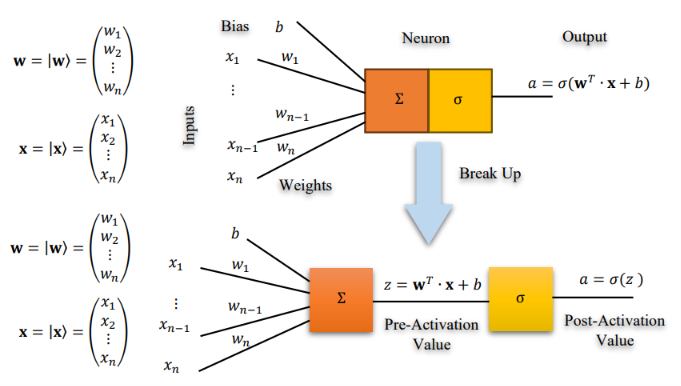
\includegraphics[width=0.8\linewidth]{Images/04_Images/1.png}
    \caption{Các giá trị trước và sau kích hoạt bên trong một nơ-ron.}
    \label{4.1}
\end{figure}
 
Về mặt toán học, một nơ-ron nhân tạo được biểu diễn như một hàm số $f: \mathbb{R}^d \to \mathbb{R}$, ánh xạ từ véc-tơ đầu vào $\mathbf{x} \in \mathbb{R}^d$ sang một giá trị đầu ra vô hướng $a \in \mathbb{R}$. 
Nơ-ron này được tham số hóa bởi một véc-tơ trọng số $\mathbf{w} = [w_1, w_2, \dots, w_d]^\top \in \mathbb{R}^d$ và một độ chệch vô hướng $b \in \mathbb{R}$. Quá trình xử lý và tạo thông tin đầu ra tại một nơ-ron nhân tạo được thực hiện thông qua hai bước liên tiếp:

\begin{enumerate}
    \item \textbf{Tính giá trị tiền kích hoạt:} Nơ-ron trước tiên thực hiện phép tổng hợp tuyến tính, giá trị tiền kích hoạt \(z\) được xác định bởi:
\begin{equation*}
    z = \sum_{i=1}^{d} w_i x_i + b
      = \mathbf{w}^{\mathsf T}\mathbf{x}+b.
\end{equation*}
Trong đó:
\begin{itemize}
    \item \(d\in\mathbb{N}\) là số chiều của véc-tơ đầu vào, tương ứng với số đặc trưng của dữ liệu đầu vào,
    
    \item \(\mathbf{x}=[x_1,x_2,\ldots,x_d]^{\mathsf T}\in\mathbb{R}^d\) là véc-tơ đầu vào, trong đó \(x_i\in\mathbb{R}\) là giá trị của đặc trưng thứ \(i\), $i = 1...d$,
    
    \item \(\mathbf{w}=[w_1,w_2,\ldots,w_d]^{\mathsf T}\in\mathbb{R}^d\) là véc-tơ trọng số, trong đó \(w_i\in\mathbb{R}\) là trọng số gán cho đặc trưng \(x_i\), $i = 1...d$,
    
    \item \(b\in\mathbb{R}\) là độ chệch, một tham số thực được sử dụng để điều chỉnh giá trị của tổng có trọng số trước khi đưa vào hàm kích hoạt.

    \item $\mathbf{w}^{\mathsf T}\mathbf{x}$ là tích vô hướng của véc-tơ trọng số $\mathbf{w}$ và véc-tơ đầu vào $\mathbf{x}$, trong đó: $$\mathbf{w}^{\mathsf T}\mathbf{x}
    =\sum_{i=1}^{d}w_i x_i;$$
    
    \item \(z\in\mathbb{R}\) là giá trị tiền kích hoạt, thu được sau khi tổng hợp các tín hiệu đầu vào theo trọng số và cộng thêm độ chệch.
    \end{itemize}
    
    \item \textbf{Tính giá trị kích hoạt:} Giá trị tiền kích hoạt \(z\) được đưa vào hàm kích hoạt \(\sigma:\mathbb{R}\rightarrow\mathbb{R}\) để tạo ra giá trị kích hoạt \(a\):
    \begin{equation*}
    a=\sigma(z)
    =\sigma\left(\mathbf{w}^{\mathsf T}\mathbf{x}+b\right).
    \end{equation*}
\end{enumerate}

Việc phân tách quá trình tính toán thành hai bước: tính giá trị tiền kích hoạt \(z\) và áp dụng hàm kích hoạt để thu được \(a\), tạo ra một biểu diễn toán học rõ ràng cho hoạt động của nơ-ron. Cách biểu diễn này cũng thuận tiện cho việc phân tích, tính toán đạo hàm trong quá trình huấn luyện mạng nơ-ron.

\paragraph{Minh họa bằng tính toán số:\\}
Xét một mẫu dữ liệu đầu vào $\mathbf{x}\in\mathbb{R}^3$, véc-tơ trọng số $\mathbf{w}\in\mathbb{R}^3$ và độ chệch $b\in\mathbb{R}$ được cho bởi:
$$\begin{aligned}
    \mathbf{x} &= \begin{bmatrix} 1 \\ -2 \\ 0.5 \end{bmatrix}, &
    \mathbf{w} &= \begin{bmatrix} 2 \\ 1 \\ -4 \end{bmatrix}, &
    b &= 1.
\end{aligned}$$
Chọn hàm kích hoạt sigmoid: $$\sigma(z)=\frac{1}{1+e^{-z}}.$$

\paragraph{Bước 1: Tính giá trị tiền kích hoạt.\\}
$$\begin{aligned}
    z &=\mathbf{w}^{\mathsf T}\mathbf{x}+b\\
    &= \begin{bmatrix}
        2&1&-4
        \end{bmatrix}
    \begin{bmatrix}
        1\\
        -2\\
        0.5
    \end{bmatrix}
    +1\\
    &=2(1)+1(-2)+(-4)(0.5)+1\\
    &=2-2-2+1\\
    &=-1.
\end{aligned}$$

\paragraph{Bước 2: Áp dụng hàm kích hoạt.}
$$\begin{aligned}
    a
    &=\sigma(z)\\
    &=\sigma(-1)=\frac{1}{1+e^{-(-1)}}=\frac{1}{1+e}\\
    &\approx\frac{1}{1+2.71828}\approx0.2689.
\end{aligned}$$
Như vậy, với véc-tơ đầu vào $\mathbf{x}$, véc-tơ trọng số $\mathbf{w}$ và độ chệch $b$ đã cho, nơ-ron tạo ra giá trị tiền kích hoạt $z=-1$ và giá trị đầu ra sau kích hoạt $a\approx0.2689$.

\begin{figure}[htbp]
\centering
\begin{tikzpicture}[
    >=Stealth,
    node distance=1.6cm,
    input_node/.style={circle, draw=green!70!black, thick, minimum size=1.1cm, font=\small},
    neuron_node/.style={circle, draw=blue!75!black, thick, minimum size=1.3cm, align=center, font=\small},
    label_text/.style={font=\footnotesize, text=black}
]
    % --- Các nút đầu vào (Input) ---
    \node[input_node] (x1) at (0, 1.8) {$x_1 = 1.0$};
    \node[input_node] (x2) at (0, 0)   {$x_2 = -2$};
    \node[input_node] (x3) at (0, -1.8){$x_3 = 0.5$};
    % --- Nhãn cột Input ---
    \node[label_text, above=0.3cm of x1] {\textbf{Đầu vào $\mathbf{x}$}};
    % --- Nơ-ron xử lý ---
    \node[neuron_node] (neuron) at (5, 0) {$\sum, \sigma$};
    \node[label_text, above=0.3cm of neuron] {\textbf{}};
    % --- Bias ---
    \node[font=\small] (bias) at (5, 1.8) {$b = 1$};
    \draw[->, thick] (bias) -- (neuron);
    % --- Kết nối từ Input tới Nơ-ron kèm trọng số -
    \draw[->] (x1) -- node[above, sloped, font=\scriptsize] {$w_1 = 2$} (neuron);
    \draw[->] (x2) -- node[above, font=\scriptsize] {$w_2 = 1$} (neuron);
    \draw[->] (x3) -- node[below, sloped, font=\scriptsize] {$w_3 = -4$} (neuron);
    % --- Đầu ra ---
    \node[right=2.2cm of neuron, font=\small, align=left] (out) {
        $z = \mathbf{w}^\top\mathbf{x} + b = -1$\\[2pt]
        $a = \sigma(-1) \approx 0.2689$
    };
    \draw[->, thick] (neuron) -- (out);
\end{tikzpicture}
\caption{Minh họa tính toán của một nơ-ron với hàm kích hoạt sigmoid.}
\end{figure}

\begin{lstlisting}[caption={Mã Python biểu diễn tính toán thủ công từng phần tử cho nơ-ron.}, language=Python]
import math

# Khoi tao
    x = [1, -2, 0.5]
    W = [2, 1, -4]
    b = 1

# 1: Tinh gia tri tien kich hoat (z)
z = ( x[0] * W[0] +  
      x[1] * W[1] + 
      x[2] * W[2] +  
      b )
      
# 2: Ap dung ham kich hoat Logistic sigmoid (a)
a = 1 / (1 + math.exp(-z))

print(f"1. Gia tri tien kich hoat (z): {z}") 
print(f"2. Gia tri dau ra sau kich hoat (a): {a}")
\end{lstlisting}

\begin{lstlisting}[caption={Mã Python biểu diễn tính toán theo véc-tơ cho nơ-ron.}, language=Python]
import numpy as np

# Ham kich hoat logistic sigmoid
def sigmoid(x: float) -> float:
    return 1.0 / (1.0 + np.exp(-x))

# Khoi tao
    x = np.array([1.0, -2.0, 0.5])
    w = np.array([2.0, 1.0, -4.0])
    b = 1.0
    
    # Buoc 1: Tinh tich vo huong w^T * x va cong them do chech b
    z = np.dot(w, x) + b
    
    # Buoc 2: Ap dung ham kich hoat sigmoid
    a = sigmoid(z)

print(f"Gia tri tien kich hoat (z): {z}")
print(f"Gia tri dau ra sau kich hoat (a): {a}")
\end{lstlisting}

\subsection{Lớp}
Trong mạng nơ-ron, \textit{lớp} là một tập các nơ-ron cùng thực hiện một phép biến đổi đối với dữ liệu đầu vào để tạo dữ liệu đầu ra. Đối với một lớp thông thường trong mạng truyền thẳng, phép biến đổi này bao gồm một phép biến đổi tuyến tính, sau đó là áp dụng hàm kích hoạt theo từng phần tử.

Xét lớp thứ $l$, nhận đầu vào là véc-tơ $\mathbf{a}^{[l-1]}\in\mathbb{R}^{n_{l-1}}$ và tạo véc-tơ đầu ra $\mathbf{a}^{[l]}\in\mathbb{R}^{n_l}.$ Quá trình tính toán của lớp được mô tả bởi:
\begin{align*}
    \mathbf{z}^{[l]} = 
    \mathbf{W}^{[l]}\mathbf{a}^{[l-1]}+\mathbf{b}^{[l]},
    \\
    \mathbf{a}^{[l]} = \sigma^{[l]}\left(\mathbf{z}^{[l]}\right).
\end{align*}
Trong đó:
\begin{itemize}
\item \(l\) là chỉ số của lớp đang xét. Nếu mạng có \(L\) lớp biến đổi, thì \(l=1,2,\ldots,L\).

\item \(n_{l-1}\) là số lượng nơ-ron của lớp \(l-1\). Với:
\[\mathbf{a}^{[l-1]}
= [a_1^{[l-1]},\ldots,a_{n_{l-1}}^{[l-1]}]^{\mathsf T}
\in\mathbb{R}^{n_{l-1}}\]
là véc-tơ đầu vào của lớp \(l\).

\item \(n_l\) là số lượng nơ-ron của lớp \(l\). Vì mỗi nơ-ron tạo ra một giá trị đầu ra nên:
\[\mathbf{a}^{[l]}=[a_1^{[l]},\ldots,a_{n_l}^{[l]}]^{\mathsf T}
\in\mathbb{R}^{n_l}.\]

\item \(\mathbf{W}^{[l]}\in\mathbb{R}^{n_l\times n_{l-1}}\) là ma trận trọng số của lớp \(l\). Phần tử \(w_{ij}^{(l)}\) biểu thị trọng số của liên kết từ nơ-ron thứ \(j\) ở lớp \(l-1\) đến nơ-ron thứ \(i\) ở lớp \(l\):

\[\mathbf{W}^{[l]}
=\begin{bmatrix}
w_{11}^{[l]} & \cdots & w_{1,n_{l-1}}^{[l]}\\
\vdots & \ddots & \vdots\\
w_{n_l,1}^{[l]} & \cdots & w_{n_l,n_{l-1}}^{[l]}
\end{bmatrix}.\]

\item \(\mathbf{b}^{[l]}\in\mathbb{R}^{n_l}\) là véc-tơ độ chệch của lớp \(l\), trong đó mỗi nơ-ron có một giá trị độ chệch:
\[\mathbf{b}^{[l]}=[b_1^{[l]},\ldots,b_{n_l}^{[l]}]^{\mathsf T}.\]

\item \(\mathbf{z}^{[l]}\in\mathbb{R}^{n_l}\) là véc-tơ giá trị tiền kích hoạt của lớp \(l\). Thành phần thứ \(i\) được xác định bởi:

\[z_i^{[l]} =\sum_{j=1}^{n_{l-1}}w_{ij}^{[l]}a_j^{[l-1]}+b_i^{[l]}.\]

\item \(\sigma^{[l]}\) là hàm kích hoạt được sử dụng tại lớp \(l\). Hàm này thường được áp dụng theo từng phần tử của véc-tơ \(\mathbf{z}^{[l]}\):
\[\mathbf{a}^{[l]}=
\sigma^{[l]}(\mathbf{z}^{[l]})=
\begin{bmatrix}
\sigma^{[l]}(z_1^{[l]})\\
\vdots\\
\sigma^{[l]}(z_{n_l}^{[l]})
\end{bmatrix}.\]
\end{itemize}

\paragraph{Trực quan bằng tính toán số.\\}
Xét một lớp có $2$ nơ-ron nhận véc-tơ đầu vào $\mathbf{x} \in \mathbb{R}^3$, ma trận trọng số $\mathbf{W} \in \mathbb{R}^{2 \times 3}$  và véc-tơ độ chệch $\mathbf{b} \in \mathbb{R}^2$ được xác định:
\[\mathbf{x} = \begin{bmatrix} 2 \\ -1 \\ 0.5 \end{bmatrix}, \qquad 
\mathbf{W} = \begin{bmatrix} 1 & -2 & 4 \\ -3 & 0 & 2 \end{bmatrix}, \qquad 
\mathbf{b} = \begin{bmatrix} -1 \\ 0.5 \end{bmatrix}.\]
Lớp này áp dụng hàm kích hoạt ReLU: $\sigma(\mathbf{z}) = \max(\mathbf{0}, \mathbf{z}).$

\paragraph{Bước 1: Thực hiện biến đổi tuyến tính.\\}
Véc-tơ tiền kích hoạt $\mathbf{z} \in \mathbb{R}^2$ được xác định thông qua phép nhân ma trận kết hợp phép cộng véc-tơ:
\[\begin{aligned}
\mathbf{z} &= \mathbf{W}\mathbf{x} + \mathbf{b} \\[3pt]
&= \begin{bmatrix} 1 & -2 & 4 \\ -3 & 0 & 2 \end{bmatrix} \begin{bmatrix} 2 \\ -1 \\ 0.5 \end{bmatrix} + \begin{bmatrix} -1 \\ 0.5 \end{bmatrix} \\[3pt]
&= \begin{bmatrix} 1(2) + (-2)(-1) + 4(0.5) \\ -3(2) + 0(-1) + 2(0.5) \end{bmatrix} + \begin{bmatrix} -1 \\ 0.5 \end{bmatrix} \\[3pt]
&= \begin{bmatrix} 2 + 2 + 2 \\ -6 + 0 + 1 \end{bmatrix} + \begin{bmatrix} -1 \\ 0.5 \end{bmatrix} \\[3pt]
&= \begin{bmatrix} 6 \\ -5 \end{bmatrix} + \begin{bmatrix} -1 \\ 0.5 \end{bmatrix} = \begin{bmatrix} 5 \\ -4.5 \end{bmatrix}.
\end{aligned}\]

\paragraph{Bước 2: Áp dụng hàm kích hoạt phi tuyến.\\}
Áp dụng hàm kích hoạt $\operatorname{ReLU}$ lên từng phần tử của $\mathbf{z}$:
\[\mathbf{a} = \sigma(\mathbf{z}) = \begin{bmatrix} \max(0, z_1) \\ \max(0, z_2) \end{bmatrix} = \begin{bmatrix} \max(0, 5) \\ \max(0, -4.5) \end{bmatrix} = \begin{bmatrix} 5 \\ 0 \end{bmatrix}.\]

\begin{figure}[H]
\centering
\begin{tikzpicture}[
    >=Stealth,
    node distance=1.8cm,
    % Phong cách các nút chuẩn học thuật
    input_node/.style={circle, draw=green!60!black, fill=green!6, very thick, minimum size=1.2cm, font=\small},
    hidden_node/.style={circle, draw=red!70!black, fill=red!6, very thick, minimum size=1.2cm, font=\small},
    % Nhãn tiêu đề
    title_label/.style={font=\bfseries\small, align=center},
    math_block/.style={font=\small, align=left}
]

    % --- 1. TIÊU ĐỀ CỘT ---
    \node[title_label] at (0, 3.2) {Lớp đầu vào\\[-1pt]{\footnotesize\itshape\color{black!70}$\mathbf{x} \in \mathbb{R}^3$}};
    \node[title_label] at (4.5, 3.2) {Lớp ẩn\\[-1pt]{\footnotesize\itshape\color{black!70}Biến đổi \& Kích hoạt}};
    \node[title_label] at (8.8, 3.2) {Biểu diễn kích hoạt\\[-1pt]{\footnotesize\itshape\color{black!70}$\mathbf{a} \in \mathbb{R}^2$}};

    % --- 2. CÁC NÚT ĐẦU VÀO (Sử dụng x làm biến số) ---
    \node[input_node] (x1) at (0, 1.8)  {$x_1 = 2.0$};
    \node[input_node] (x2) at (0, 0.0)  {$x_2 = -1$};
    \node[input_node] (x3) at (0, -1.8) {$x_3 = 0.5$};


    % --- 3. CÁC NÚT TẦNG ẨN ---
    \node[hidden_node] (n1) at (4.5, 1.0)  {$\sum, \sigma$};
    \node[hidden_node] (n2) at (4.5, -1.0) {$\sum, \sigma$};

    % --- 4. LIÊN KẾT ĐẦY ĐỦ (Cập nhật để kết nối với các nút x) ---
    \foreach \i in {1,2,3} {
        \foreach \j in {1,2} {
            \draw[->, draw=black!45, line width=0.7pt] (x\i) -- (n\j);
        }
    }
    % Nhãn ma trận trọng số ở giữa
    \node[font=\footnotesize, text=black!60, fill=white, inner sep=2pt] at (2.25, 0) {$\mathbf{W}, \mathbf{b}$};

    % --- 5. MŨI TÊN VÀ KHỐI KẾT QUẢ ĐẦU RA ---
    % Nhánh 1 (Cập nhật h -> x trong công thức)
    \draw[->, very thick, draw=black!75] (n1) -- (6.3, 1.0);
    \node[math_block, anchor=west] at (6.5, 1.0) {
        $\begin{aligned}
            z_1 &= \mathbf{w}_1^\top\mathbf{x} + b_1 = 5 \\[2pt]
            a_1 &= \max(0, z_1) = \mathbf{5}
        \end{aligned}$
    };

    % Nhánh 2 (Cập nhật h -> x trong công thức)
    \draw[->, very thick, draw=black!75] (n2) -- (6.3, -1.0);
    \node[math_block, anchor=west] at (6.5, -1.0) {
        $\begin{aligned}
            z_2 &= \mathbf{w}_2^\top\mathbf{x} + b_2 = -4.5 \\[2pt]
            a_2 &= \max(0, z_2) = \mathbf{0}
        \end{aligned}$
    };

\end{tikzpicture}
\caption{Cơ chế tính toán của một lớp có 2 nơ-ron.}
\end{figure}

\begin{lstlisting}[caption={Mã Python biểu diễn tính toán theo ma trận - véc-tơ cho một lớp.}, language=Python]
import numpy as np

# Ham kich hoat ReLU: f(x) = max(0, x)
def relu(x: np.ndarray) -> np.ndarray:  
    return np.maximum(0, x)

# Khoi tao vec-to dau vao, ma tran trong so va do chech
x = np.array([2.0, -1.0, 0.5])
W = np.array([
    [ 1.0, -2.0,  4.0],
    [-3.0,  0.0,  2.0]
  ])
b = np.array([-1.0, 0.5])
    
# Buoc 1: Tinh vec-to tien kich hoat z = Wx + b
z = np.dot(W, x) + b
    
# Buoc 2: Ap dung ham kich hoat ReLU
a = relu(z)
    
print(f"Vec-to tien kich hoat (z):\n{z}")
print(f"\nVec-to dau ra sau kich hoat ReLU (a):\n{a}")
\end{lstlisting}